\documentclass{beamer}
\usetheme{Boadilla}
\usepackage{polski}
\usepackage[utf8]{inputenc}
\title{BTS Maintenance System }
\subtitle{Wykorzystane technologie}
 \author{Michał Błach, Kacper Szewczyk}
%\institute{Slyboots \& Zawodnik Company}
\date{\today}
\setbeamercovered{transparent}
\begin{document}
\begin{frame}
\titlepage
\end{frame}
\begin{frame}
\tableofcontents
\end{frame}

\section{Aplikacja kliencka}

\subsection{Projektowanie aplikacji i problemy z tym związane}
\begin{frame}{Znana sytuacja ?}
     \begin{columns}[T] % contents are top vertically aligned
      \begin{column}[T]{8cm} % alternative top-align that's better for graphics
          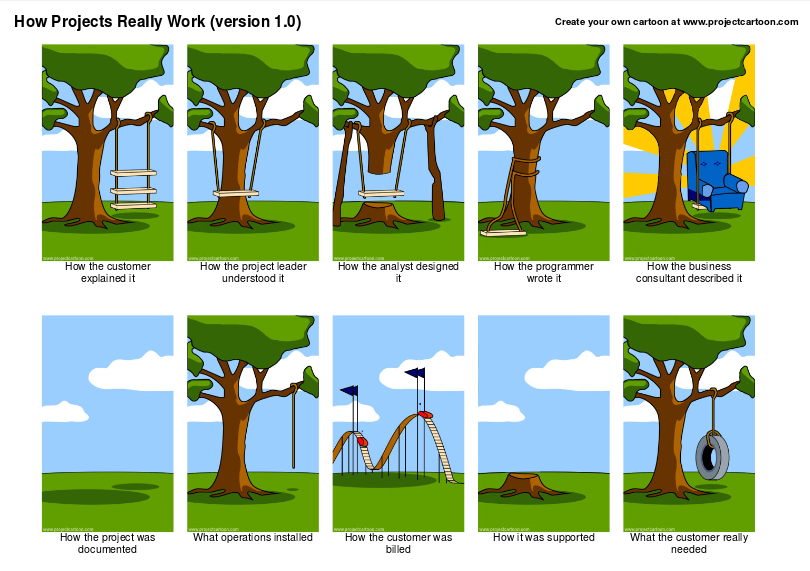
\includegraphics[width=8cm]{how_works.png}
     \end{column}
     \begin{column}[T]{4cm} % each column can also be its own environment
     \begin{block}<1->{Nowy projekt/zlecenie}
	Rozpoczynamy nowy projekt startup.\\
	Po długich rozmowach z potencjalnymi klientami udaje nam się skonkretyzować specyfikacje projektu.
	Rozpoczynamy implementacje, po czym okazuje się, że \dots 
\end{block}
     \end{column}
     \end{columns}
\end{frame}


\begin{frame}{Znana sytuacja ?}
     \begin{columns}[T] % contents are top vertically aligned
     
          \begin{column}[T]{7cm} % each column can also be its own environment
    % \begin{block}<1->{Nowy projekt/zlecenie}
   % \framesubtitle{<subtitle>}
	\begin{itemize}
    \item<1-> Firma zmieniła telefony służbowe pracowników
    \item<2-> Project Manager pracujący u klienta używa innego OS.
    \item<3-> Zaszla potrzeba użytkowania aplikacji na Notebook-u/Laptopie
    \item<4-> \dots
    \end{itemize}
%\end{block}
     \end{column}
      \begin{column}[T]{5cm} % alternative top-align that's better for graphics
          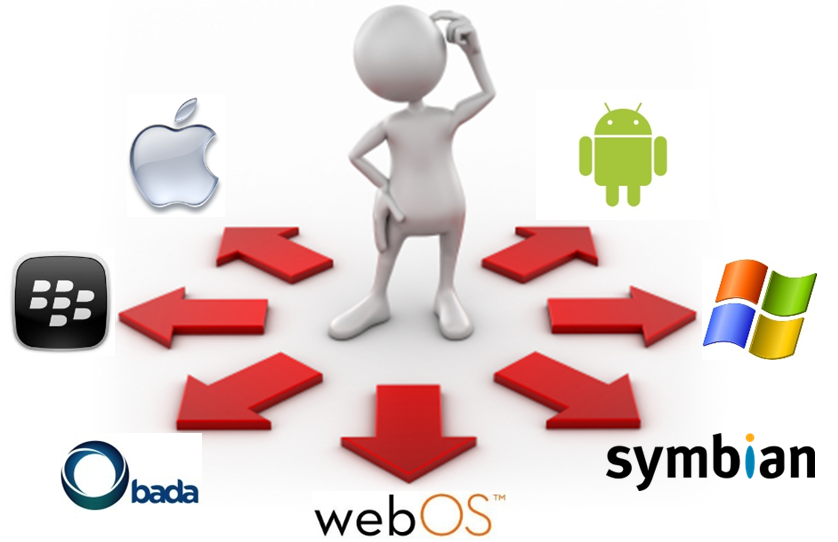
\includegraphics[width=5cm]{mobile.png}
     \end{column}
     \end{columns}
\end{frame}

\begin{frame}{Klasyczne rozwiązanie}
     \begin{columns}[T] % contents are top vertically aligned
      
     \begin{column}[T]{6cm} % each column can also be its own environment
     \begin{block}<1->{Zalety}
			\begin{itemize}
    \item<1-> Większa wydajność aplikacji
    \item<2-> Łatwy dostęp do interface-ów/urządzeń w urządzeniu, poprzez natywne odwołania
    \item<3-> \dots
    \end{itemize}
	\end{block}
     \end{column}
     \begin{column}[Tc]{6cm} % alternative top-align that's better for graphics
          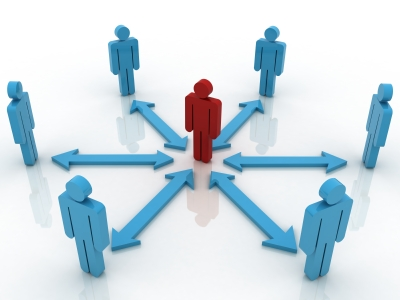
\includegraphics[width=6cm]{multi.jpg}
     \end{column}
     \end{columns}
\end{frame}


\begin{frame}{Klasyczne rozwiązanie}
     \begin{columns}[T] % contents are top vertically aligned
      
     \begin{column}[T]{6cm} % each column can also be its own environment
     \begin{block}<1->{Wady}
			\begin{itemize}
    \item<1-> Zatrudnienie wielu zespołów programistów do implementacji projeku na każdej 
    platformie.
    \item<2-> Powielanie tego samego kodu.
    \item<3-> Utrzymywanie wiele projektów, co wiąże sie z zatrudnieniem wielu
    ludzi, z powodów czasowych i technologicznych.
    \item<4-> Niejednolitość interface na każdej platformie.
    \item<5-> \dots
    \end{itemize}
	\end{block}
     \end{column}
     \begin{column}[Tc]{6cm} % alternative top-align that's better for graphics
          
\includegraphics[width=6cm]{busy.jpg}
     \end{column}
     \end{columns}
\end{frame}

\subsection{Dostępne frameworki}
\begin{frame}
\frametitle{Corona}
\begin{figure}
 
\includegraphics[width=12cm,valign=t]{corona.png}
 \end{figure}
 \begin{block}{Opis z oficjalnej strony }
Corona's extensive API library enables everything from animation to networking with just a few lines of code. Whether you're building games or business apps, you see changes instantly in the Corona Simulator and can iterate extremely quickly. Development is done in Lua, a lightning-fast and easy to learn scripting language. Couple Corona with Corona Editor and/or Composer GUI you'll achieve even faster workflow. 
 \end{block}
\end{frame}

\begin{frame}
\frametitle{QT}
\begin{figure}
 
\includegraphics[width=7cm,valign=t]{qt.png}
 \end{figure}
 \begin{block}{Opis z oficjalnej strony }
You can write and recycle Qt application and device UI code to run on all your target devices. You can take your applications everywhere: embedded, desktop and mobile platforms. Qt lets you future-proof your “things” by making them platform independent. Should you want diversity between platforms, like a responsive UI design for different screen sizes, this is simple to implement with Qt, as well.
 \end{block}
\end{frame}

\subsection{Cordova}

\begin{frame}
\frametitle{Cordova}

\begin{figure}
 
\includegraphics[width=9cm,valign=t]{cordova.png}
 \end{figure}
 \begin{block}{Opis z oficjalnej strony }
Cordova wraps your HTML/JavaScript app into a native container which can access the device functions of several platforms. These functions are exposed via a unified JavaScript API, allowing you to easily write one set of code to target nearly every phone or tablet on the market today and publish to their app stores. 
 \end{block}
\end{frame}
\begin{frame}
\frametitle{Cordova}
\framesubtitle{Wspierane SO}
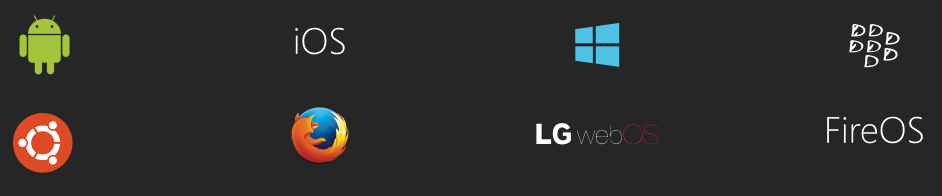
\includegraphics[width=12cm,valign=t]{sup_plat1.png}


\end{frame}

\begin{frame}
\frametitle{Cordova}
\framesubtitle{Obsługa urządzeń}


      
    
          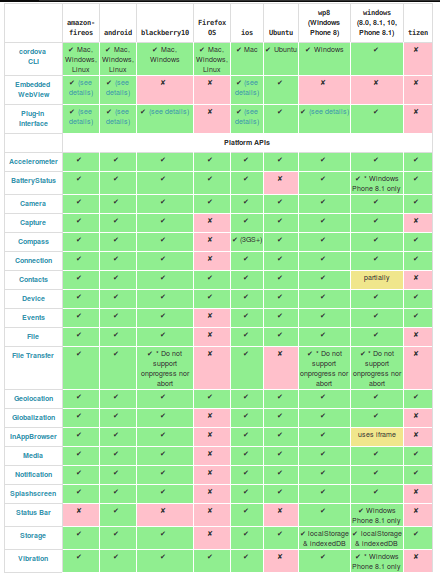
\includegraphics[height=8cm,valign=t]{supp_plat.png}

\end{frame}
\begin{frame}
\frametitle{Cordova}
\framesubtitle{Szybki start}
\begin{block}<1->{Pierwsze kroki}
%\begin{itemize}
  \visible<1->{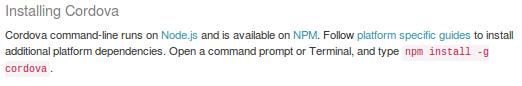
\includegraphics[width=8cm]{fs1.png}}
    \visible<2->{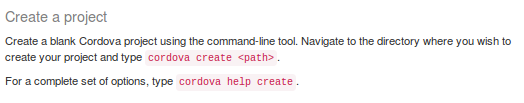
\includegraphics[width=8cm]{fs2.png}}
      \visible<3->{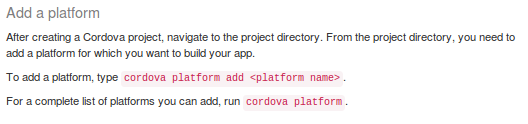
\includegraphics[width=8cm]{fs3.png}}
        \visible<4->{
\includegraphics[width=8cm]{fs4.png}}
%	\only<2>  {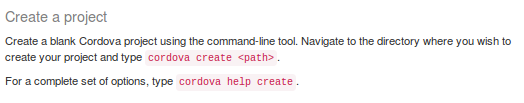
\includegraphics[height=1cm,valign=t]{fs2.png}} 	
%	\only<3>  {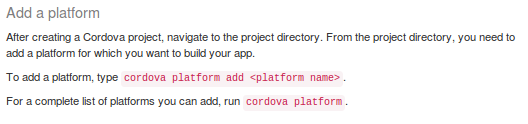
\includegraphics[height=1cm,valign=t]{fs3.png}}
%	\only<4>  {
\includegraphics[height=1cm,valign=t]{fs4.png}}
    
 %   \end{itemize}
\end{block}
\end{frame}
\subsubsection{HTML5}
\begin{frame}
\frametitle{HTML5}


\begin{columns}[T] % contents are top vertically aligned
      
     \begin{column}[T]{7cm} % each column can also be its own environment
    \begin{block}<1->{Nowości w HTML5 }
 
\begin{itemize}
\item  Nowe tagi: section, article, header, footer, nav, video, audio, mark, progress, ...\\
\item Nowe typy pól "input": tel, search, url, email, datetime, date, month, week, time, datetime-local, number, range, color.
\item Nowe atrybuty elementów formularzy: autofocus, required, autocomplete, min, max, multiple, pattern, step, ...
\item Możliwość osadzenia MathML i SVG bezpośrednio w dokumencie, zupełnie jak w XHTML


\end{itemize}
\end{block}
     \end{column}
     \begin{column}[Tc]{5cm} % alternative top-align that's better for graphics
     \begin{figure}[!ht]

  \centering
  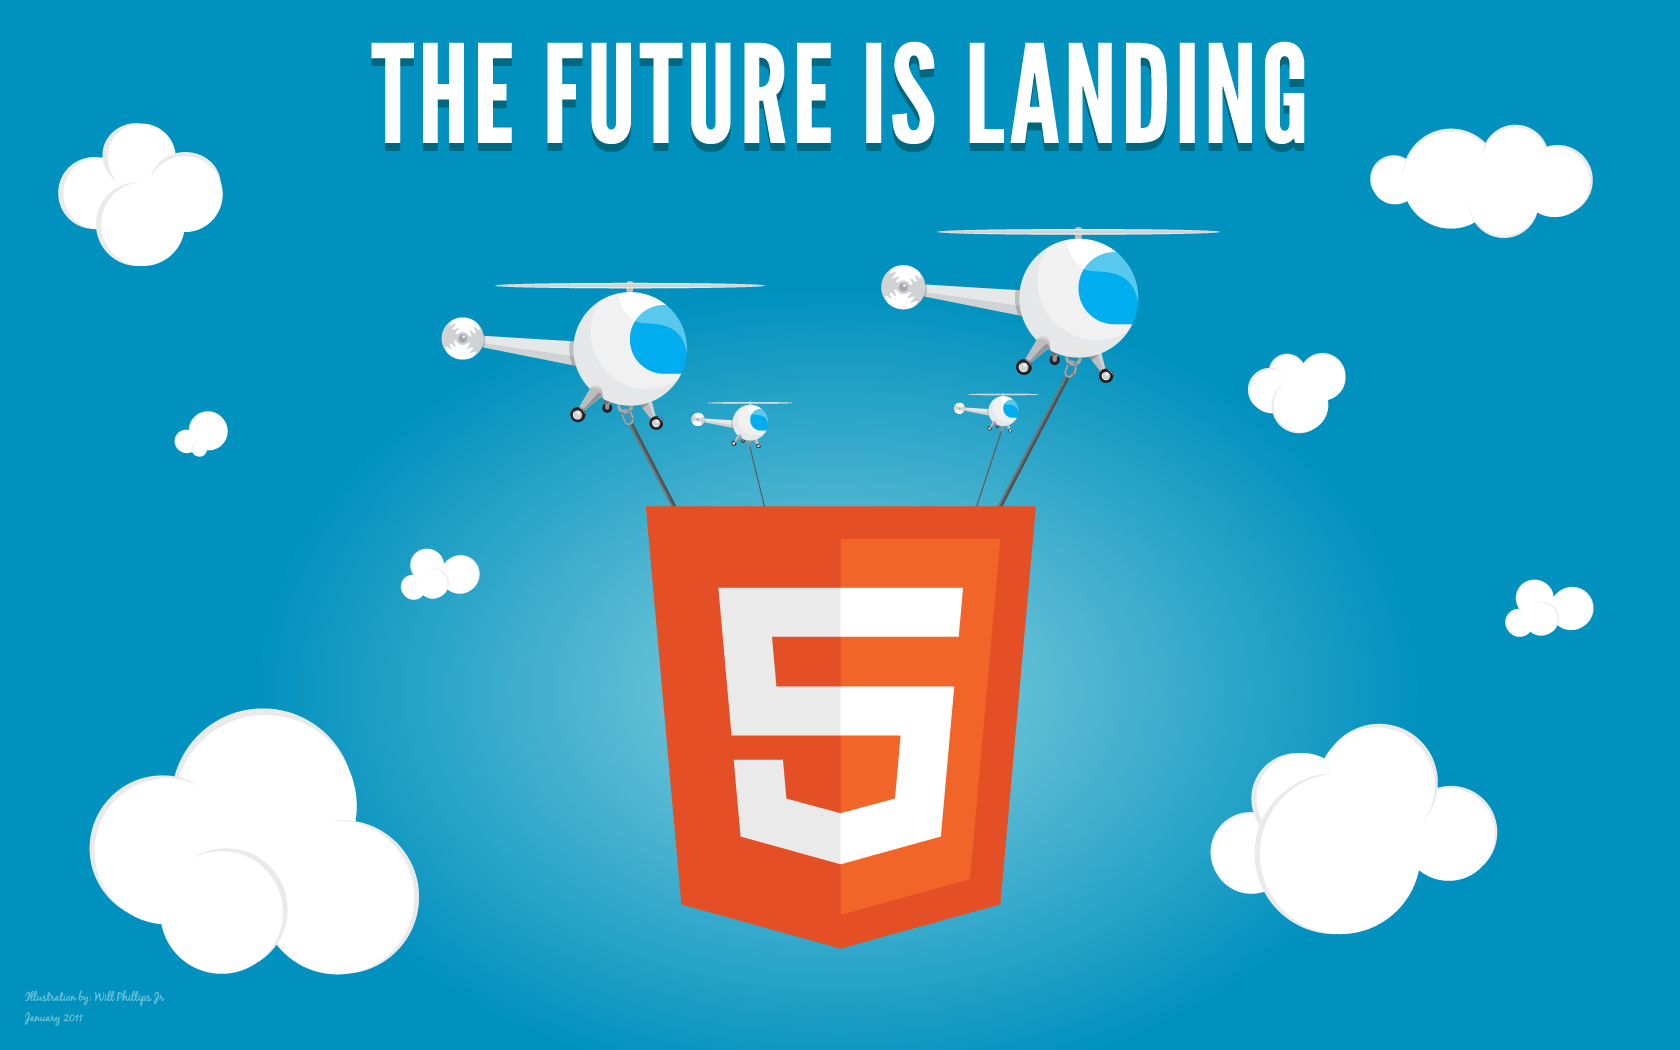
\includegraphics[width=5cm]{html5.png}
\end{figure}
          
     \end{column}
     \end{columns}
     
     
     
 
\end{frame}

\begin{frame}
\frametitle{HTML5}

\begin{block}<1->{Nowości w API}
\begin{itemize}
\item Rysowanie 2D z nowym elementem canvas,
\item  WebGL (port OpenGL dla przeglądarek),
\item  API dla odtwarzania audio i video,
\item  API dla aplikacji offline,
\item  API, pozwalające zarejestrować aplikację WEB jako protokół lub media type,
\item  API przeciągnij i upuść, z atrybutem draggable,
\item  API do obsługi przycisku wstecz (History API),

\end{itemize}
\end{block}
\end{frame}

\begin{frame}
\frametitle{HTML5}

\begin{block}<1->{Nowości w API c.d}
\begin{itemize}
\item  API pamięci (storage) pozwalające na przechowywanie danych pomiędzy przeładowaniami strony,
\item  Microdata – przechowywanie danych w atrybutach
\item  Geolokalizacja,
\item  Web Sockets (dwukierunkowa komunikacja z serwerem),
\item  Komunikacja między stronami (np. można wysyłać informację do strony znajdującej się w ramce).
\item  Nowa wersja XMLHttpRequest umożliwiająca upload plików oraz monitorowanie postępu
\item  File API – dostęp do systemu plików po stronie klienta
\end{itemize}
\end{block}
\end{frame}

%\subsubsection{CSS3}
%\begin{frame}
%\frametitle{Frame1}
%\end{frame}
\subsubsection{Java Script}
\begin{frame}
\frametitle{Java Script}
     \begin{columns}[T] % contents are top vertically aligned
      
     \begin{column}[T]{6cm} % each column can also be its own environment
    \begin{block}<1->{Frameworki}
			\begin{itemize}
    \item<1-> AngularJS
    \item<2->  EmberJS
    \item<3->  Backbone
    \item<4->  Kendo UI
    \item<5-> Monaca
    \item<6->  ReactJS
    \item<6-> Sencha Touch
    \item<6->  jQuery Mobile
    \item<5-> \dots
\end{itemize}
\end{block}
     \end{column}
     \begin{column}[T]{6cm} % alternative top-align that's better for graphics
          
\includegraphics[width=6cm]{js.png}
     \end{column}
     \end{columns}
     
     

\end{frame}
\section{Zewnętrzny serwer do synchronizacji danych}


\subsection{JBoss WILDFLY}
\begin{frame}
\frametitle{JBoss WILDFLY}

\includegraphics[width=6cm]{wildfly.jpg}



\end{frame}
\subsection{Jęzki programowania i frameworki}
\subsubsection{Java 1.8 }
\begin{frame}
\frametitle{Java 1.8 nowości }
\framesubtitle{lambda}
\begin{itemize}


\item 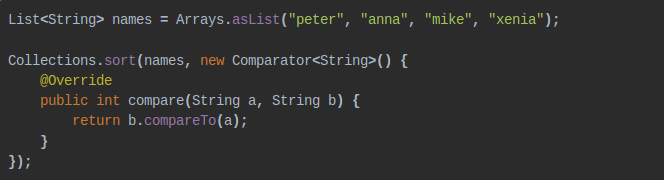
\includegraphics[width=12cm]{lambda1.png}
\item  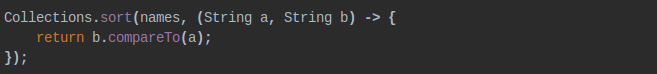
\includegraphics[width=12cm]{lambda2.png}
  \end{itemize}
  \end{frame}
  \begin{frame}
\frametitle{Java 1.8 nowości }
\framesubtitle{referencje do metod i konstruktorow}
    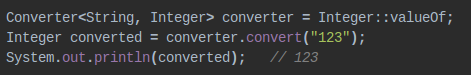
\includegraphics[width=12cm]{method_ref.png}
    \end{frame}
    \begin{frame}
\frametitle{Java 1.8 nowości }
\framesubtitle{predykaty}
     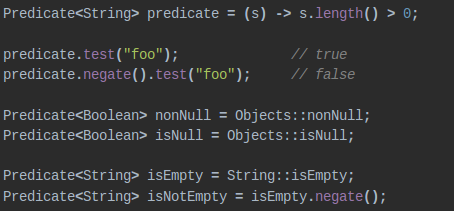
\includegraphics[width=12cm]{predicate.png}
     \end{frame}
     \begin{frame}
\frametitle{Java 1.8 nowości }
\framesubtitle{optionale}
     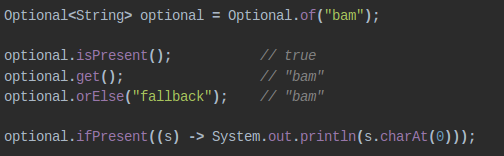
\includegraphics[width=10cm]{optional.png}
   \end{frame}  
     \begin{frame}
\frametitle{Java 1.8 nowości }
\framesubtitle{filtry}
      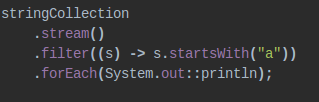
\includegraphics[width=10cm]{filter.png}
      \end{frame}
      \begin{frame}
\frametitle{Java 1.8 nowości }
\framesubtitle{mapowanie}
      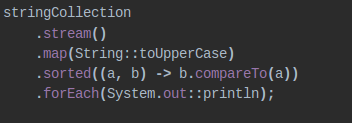
\includegraphics[width=10cm]{map.png}
\end{frame}
%\begin{itemize}
%    \item<1-1> Default Methods for Interfaces
    
%    \item<2-> Lambda expressions
%    \item<3-> Method and Constructor References
%    \item<4-> Predicates are boolean-valued functions of one argument. The interface contains various default %methods for composing predicates to complex logical terms (and, or, negate)
%    \item<5-> Optionals
%    \item<6-> Streams
%    \item<6-> Clock
%    \item<5-> \dots
%\end{itemize}

\subsubsection{JAX-RS Jersey}
\begin{frame}
\frametitle{JAX-RS Jersey}

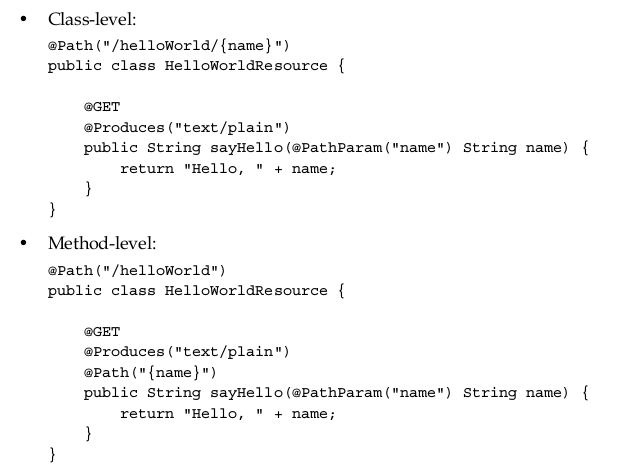
\includegraphics[width=10cm]{jax.png}
\end{frame}


\end{document}
